\chapter{Піксель та Воксель. Загальні відомості}\label{cha:pixel_voxel}
Кожен піксель має певні розміри (XY, де переважно X = Y) і певне значення відтінку сірого, щоби описати матеріал, який він представляє.
Зображення розташовані на певній відстані (Z).
Ця відстань надає пікселям певної глибини.
VOlume piXEL називається вокселем, він має розміри XYZ.\cite{img_operators:4}
Тобто додаючи третій параметр до значення ми розширюємо поняття.

Для того щоби краще зрозуміти воксель, переглянемо інформацію про піксель.

Піксель на рисунку 1. можна сприймати як контейнр, який збирає світло або електрони, залежно від типу використовуваного детектора.
Один піксель на зображенні охоплює якусь відстань у фізичному світі.
Наприклад, на рисунок 1. стрілки вказують ширину та висоту пікселя, розміщеного поруч із трьома іншими пікселями.
У цьому випадку ширина та висота цього пікселя становлять 0,5 мм.

\begin{figure}
    \label{fig:image1}
    \centering
    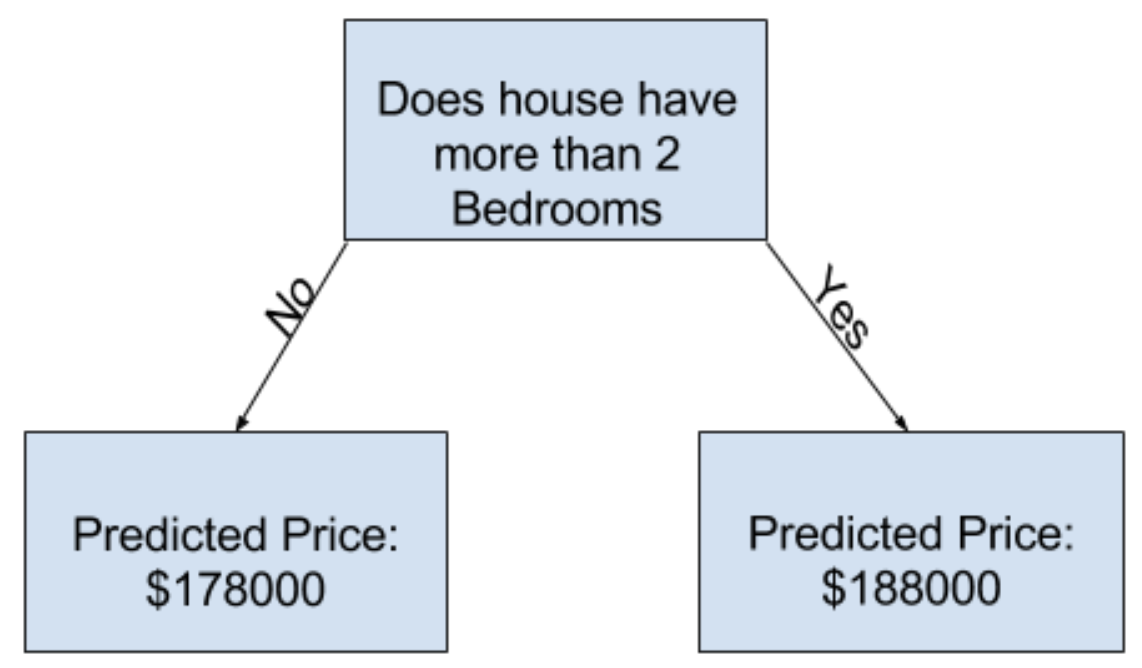
\includegraphics[scale=0.5]{image1.png}

    Рис. 1. Фізичне відображення пікселя.
\end{figure}

Таким чином, у фізичному просторі подолання відстані 0,5 мм еквівалентно подоланню 1 пікселя в піксельному просторі.
З усіх практичних цілей можна припустити, що детектори мають квадратні пікселі, тобто ширина та висота пікселів однакові.

Розмір пікселів може бути різним для різних методів зображення та різних детекторів.
Наприклад, розмір пікселів більший для CT порівняно з mikro-CT.

\section{Воксель в медицинi.}\label{sec:voxel_med}
У медичній та мікроскопічній зйомках частіше отримують тривимірні зображення.
У таких випадках розмір пікселя матиме третій вимір, а саме глибина пікселів.
Термін піксель, як правило, застосовується до 2D і замінюється вокселем у 3D-зображеннях.

Більшість поширених форматів зображень, таких як DICOM, nifti та деякі формати зображень з мікроскопом, містять розмір вокселів у своєму заголовку.\cite{img_operators:4}
Отже, коли такі зображення читаються у програмі візуалізації або обробки зображень, може бути здійснений точний аналіз та візуалізація.
Але якщо зображення не містить інформації в заголовку або якщо програма візуалізації чи обробки зображень не може правильно прочитати заголовок, важливо використовувати правильний розмір вокселя для аналізу.
